\pstart 
%Zeitz auskommentiert \begin{wrapfigure}{l}{0.1\textwidth}                    
%                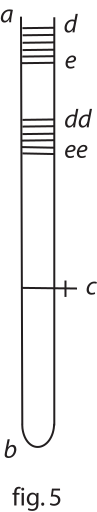
\includegraphics[width=0.1\textwidth]{images/37_4_114v}\\\textit{[Fig. 6]}
%                        %\caption{Bildbeschreibung}
%                        \end{wrapfigure}
%                        %@ @ @ Dies ist eine Abstandszeile - fuer den Fall, dass mehrere figures hintereinander kommen, ohne dass dazwischen laengerer Text steht. Dies kann zu einer Fahlermeldung fuehren. @ @ @ \\
[114 v\textsuperscript{o}] \edlabel{114vseq}\edtext{\textso{Prop. 5.}}{\lemma{seq.}\xxref{114rseq}{114vseq}\Afootnote{ \textit{ (1) }\ \textso{Exper. 5.} \textit{ (2) }\ \textso{Prop. 5.} \textit{ L}}} Ostensum est prop. praecedenti \edtext{si pondus et Elasticum liquida}{\lemma{praecedenti}\Afootnote{ \textit{ (1) }\ in liquidis \textit{ (2) }\ si pondus  \textbar\ pariter \textit{ gestr.}\ \textbar\  et Elasticum liquida \textit{ L}}} sint, nihil referre, quanta sit capacitas \edtext{alterutrius si}{\lemma{alterutrius}\Afootnote{\textbar~sed \textit{ gestr.}\ \textbar\ si \textit{ L}}} vero solida sint, eo casu nihil refert quanta sit capacitas seu magnitudo Elaterii\protect\index{Sachverzeichnis}{elaterium}, dummodo homogeneum sit, refert vero quantum sit pondus\protect\index{Sachverzeichnis}{pondus}. Cessat enim ratio illa Hydrostatica\protect\index{Sachverzeichnis}{hydrostatica} quam a Tuborum amplitudine per motum compensata petivimus. Propositio ergo haec erit. Si eadem vis (pondus\protect\index{Sachverzeichnis}{pondus} an Elaterium\protect\index{Sachverzeichnis}{elaterium} nihil refert) Elateriis\protect\index{Sachverzeichnis}{elaterium} diversis homogeneis, magnitudine differentibus applicetur, spatia corpori compresso ademta aut tenso addita \edtext{vel corpora compresso addita, tenso ademta}{\lemma{}\Afootnote{vel [...] ademta \textit{ erg.} \textit{ L}}} aequalia erunt, etsi ipsa corpora Elastica\protect\index{Sachverzeichnis}{corpus!elasticum} sint \edtext{magnitudine}{\lemma{}\Afootnote{magnitudine \textit{ erg.} \textit{ L}}} inaequalia. \edtext{Dummodo non sint inaequaliter Elastica}{\lemma{}\Afootnote{Dummodo non sint inaequaliter Elastica \textit{ erg.} \textit{ L}}} cujus propositionis veritas hoc Experimento comprobari aut falsitas revinci potest. Esto Tubus \edtext{\textit{ab}}{\lemma{}\Afootnote{\textit{ab} \textit{ erg.} \textit{ L}}} 
                         infra clausus in \textit{b}  in cujus medio alicubi, ut in \textit{c} \edtext{sit}{\lemma{}\Afootnote{sit \textit{ erg.} \textit{ L}}}. Epistomium\protect\index{Sachverzeichnis}{epistomium} quod modo aperiri, modo claudi possit, \edtext{non ut intret aer externus, sed ut communicatio inter duas Tubi partes \textit{ec} et \textit{cb} modo permittatur, modo negetur.}{\lemma{}\Afootnote{non [...] inter \textit{ (1) }\ duos Tubos \textit{ (2) }\ duas [...] negetur. \textit{ erg.} \textit{ L}}} \edtext{Aperiatur Epistomium}{\lemma{Aperiatur}\Afootnote{ \textit{ (1) }\ primum \textit{ (2) }\ Epistomium \textit{ L}}}, Mercuriusque \protect\index{Sachverzeichnis}{mercurius} \textit{de} descendat \edtext{quousque potest in}{\lemma{quousque}\Afootnote{ \textit{ (1) }\ lubet in \textit{ (2) }\ potest in \textit{ L}}} \textit{ddee}. Ajo si Epistomium\protect\index{Sachverzeichnis}{epistomium} non fuisset apertum, cum descenderet sed clausum, seu si Tubus fuisset non longitudinis \textit{eb} sed solum longitudinis \textit{ec}. Mercurium\protect\index{Sachverzeichnis}{mercurius} nihilominus descensurum fuisse per altitudinem eandem \textit{edd} seu non ultra quam ex \textit{de} in \textit{ddee}. \edtext{Demonstratio}{\lemma{\textit{ddee}.}\Afootnote{ \textit{ (1) }\ Hujus rei ratio \textit{ (2) }\ Demonstratio \textit{ L}}} haec est: spatium ab aere Tubi \edtext{majoris, seu totius \textit{ab}}{\lemma{}\Afootnote{majoris, seu totius \textit{ab} \textit{ erg.} \textit{ L}}} initio, ante Mercurii\protect\index{Sachverzeichnis}{mercurius} descensum occupatum est \textit{eb} \edtext{post descensum}{\lemma{\textit{eb}}\Afootnote{ \textit{ (1) }\ si Tubus est major, \textit{ec} si minor \textit{ (2) }\ post descensum \textit{ L}}} \textit{eeb}. Ergo spatium descensu ablatum est \textit{e ee} aer ergo qui in spatio \textit{eee} fuit locum in reliquo aere \textit{ee b} quaerit, seu reliquus aer totus comprimitur aequaliter, ut enim aer loco suo exul in proximo hospitium quaerit, ita proximus in sibi proximum intrare conatur ut locum faciat novo: omnes ergo aeque sufferunt, seu aer exul per caeteros aequaliter distribuitur. Hinc \edtext{quanto major est aer comprimendus}{\lemma{quanto}\Afootnote{ \textit{ (1) }\ major est locus \textit{ (2) }\ major est aer comprimendus \textit{ L}}} \edtext{seu materia}{\lemma{}\Afootnote{seu materia \textit{ erg.} \textit{ L}}}, tanto minor est compressio\protect\index{Sachverzeichnis}{compressio} partium singularum; et quanto minor est aer seu materia, tanto major est gradus\protect\index{Sachverzeichnis}{gradus} \edtext{compressionis\protect\index{Sachverzeichnis}{compressio}. Summa}{\lemma{compressionis.}\Afootnote{ \textit{ (1) }\ Duo autem \textit{ (2) }\ Summa \textit{ L}}} compressionis\protect\index{Sachverzeichnis}{compressio} fit ex ductu materiae in gradum. Materia aucta minuitur gradus, et contra, \edtext{constat enim si duo sunt factores v.g. 2. et 8. et uno minuto verbi gratia, dimidiato alter proportionaliter augeatur, v.g. duplicetur ut 1. et 16. vel 4. et 4. factum semper esse eundem. Eadem ergo est summa compressionis}{\lemma{contra,}\Afootnote{ \textit{ (1) }\ ergo eadem est summa compressionis\protect\index{Sachverzeichnis}{compressio|textit} seu idem effectus pondere per eandem altitudinem descendente, seu tantundem aeris \textit{ (2) }\ constat [...] 2.  \textbar\ et \textit{ erg.}\ \textbar\ 8. [...] compressionis \textit{ L}}}, \edtext{ac proinde eadem difficultas sive}{\lemma{compressionis,}\Afootnote{ \textit{ (1) }\ seu proinde \textit{ (2) }\ sive eadem difficultas \textit{ (3) }\ ac proinde eadem difficultas sive \textit{ L}}} idem aer exul in \edtext{majorem sive in minorem}{\lemma{in}\Afootnote{ \textit{ (1) }\ plures \textit{ (2) }\ majorem sive in minorem \textit{ L}}} \edtext{comprimendum}{\lemma{minorem}\Afootnote{ \textit{ (1) }\ minuendum \textit{ (2) }\ comprimendum \textit{ L}}} distribuatur, ut autem idem sit aer exul, eodem descensu opus est. Ergo quantaecunque longitudinis fiat Tubus \textit{ab} Mercurius\protect\index{Sachverzeichnis}{mercurius} \textit{de} non descendet, nisi usque ad \textit{ddee} seu idem erit spatium ademtum \edtext{\textit{eee}. Demonstratio est}{\lemma{\textit{eee}}\Afootnote{ \textit{ (1) }\ quod erat demonstrandum. \textit{ (2) }\ . Demonstratio est \textit{ L}}} irrefragabilis, sed ut harmonia cum caeteris naturae principiis intellecta fiat illustrior, haec adjungenda duxi.  
                         \pend 